\begin{tikzpicture}[inner sep=0pt,outer sep=0pt]
\draw (0,-1) node[scale=.75] (V) {\input{\mainfolder/DrawingElements/CircuitElements/voltagesource.tex}};
\draw (1,0) node (R1) {\begin{tikzpicture}
\draw[very thick] (0,0) -- ++(.37,0);
\draw[very thick] (1,0) node[rectangle,draw,minimum width=.5in,minimum height=.1in] {};
\draw[very thick] (1.65,0) -- ++(.37,0);
\end{tikzpicture}
};
\draw (2,-1) node (R2)[rotate=90] {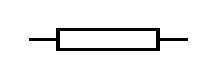
\begin{tikzpicture}
\draw[very thick] (0,0) -- ++(.37,0);
\draw[very thick] (1,0) node[rectangle,draw,minimum width=.5in,minimum height=.1in] {};
\draw[very thick] (1.65,0) -- ++(.37,0);
\end{tikzpicture}
};



\draw (R1) node[above=6pt] {$Z_{1}(s)$};
\draw (R2) node[left=6pt] {$Z_{2}(s)$};
\draw (V) node[left=12pt] {$V_{in}(s)$};
\draw (R2) ++(1,0) node {$V_{out}(s)$};
\draw (R2) ++(1,1) node {$+$};
\draw (R2) ++(1,-1) node {$-$};
\draw[very thick] (V.90) |- (R1.180);
\draw[very thick] (R1.0) -| (R2.0);
\draw[very thick] (R2.180) -| (V.-90);

\draw (1,-2.75) node {$V_{out}(s) = \frac{Z_{2}(s)}{Z_{1}(s)+Z_{2}(s)}V_{in}(s)$};

%\draw (6.1,.75) node[above] {$+$};
%\draw (7,.75) node[above] {$X(s)$};
%\draw (7.9,.75) node[above] {$-$};

\end{tikzpicture}